\section{TEORİK ALTYAPI}

\subsection{Işığa Bağımlı Dirençler (LDR)}

LDR'ler, foto dirençler olarak da bilinir, üzerine düşen ışığın yoğunluğuna bağlı olarak direnç değişikliği gösteren pasif elektronik bileşenlerdir. Bu özellik, onları ışık algılama, otomatik aydınlatma sistemleri ve fotovoltaik hücreler gibi çeşitli uygulamalarda önemli hale getirir \cite{perkinelmer2001}.

\subsubsection{Temel Çalışma Prensibi}
Bir LDR'nin çalışması, üzerine düşen fotonların enerji almasıyla gerçekleşen fotoelektrik etkiye dayanır. Bu etki, yeterli enerjiye sahip fotonlar, yarı iletken malzemenin (genellikle kadmiyum sülfür (CdS) veya kadmiyum selenyür (CdSe) gibi) yüzeyine çarptığında meydana gelir. Işık tarafından emilen enerji, malzemedeki elektronları uyarır, serbest hareket etmelerine izin verir ve böylece bileşenin direncinin azalmasına neden olur. Işık yoğunluğu (\(I\)) ile direnç (\(R\)) arasındaki ilişki \eqref{eq:R_LDR}'deki gibidir:

\begin{equation}
R \propto \frac{1}{I}
\label{eq:R_LDR}
\end{equation}

Işık yoğunluğu arttıkça, direnç düşer; ışık yoğunluğu azaldıkça direnç artar \cite{khan2005introduction}.

\subsubsection{LDR Empirik Direnç Formülü}

Bir LDR'nin direnci, \( R_{LDR} \), üzerine düşen ışık yoğunluğuyla ters orantılıdır. Bu ilişki, empirik bir formülle tanımlanabilir:

\begin{equation}
R_{LDR} = \frac{A}{L^{\gamma}}
\label{eq:LDR_emp}
\end{equation}

Burada:
\begin{itemize}
    \item \( R_{LDR} \), LDR'nin direncidir.
    \item \( A \), LDR'ye ve malzeme özelliklerine özgü bir sabittir.
    \item \( L \), lüks (lx) cinsinden ölçülen ışık yoğunluğudur.
    \item \( \gamma \), genellikle 0.7 ile 1.0 arasında değişen bir katsayıdır ve LDR'nin özel malzemesine ve tasarımına bağlıdır.
\end{itemize}

\eqref{eq:LDR_emp}, ışık yoğunluğu \( L \) arttıkça direncin \( R_{LDR} \)'nin azaldığını gösterir \cite{perkinelmer2001}.


Yarı iletken malzeme seçimi, LDR'lerin performansını etkiler. Görünür ışık spektrumundaki hassasiyeti nedeniyle CdS sıkça kullanılır. Yarı iletkenin enerji band aralığı, algılayabileceği ışık dalga boyunu belirler. CdS için band aralığı yaklaşık 2.35 eV olup, 500-575 nm aralığındaki dalga boylarına duyarlılık gösterir \cite{nagesh1979photoconductivity}.

\subsubsection{Spektral Yanıt}
LDR'ler belirli bir spektral yanıt gösterir; bu, farklı dalga boylarına farklı tepkiler verdikleri anlamına gelir.

\begin{comment}
    \ref{fig:spektralyanıt}de bazı materyallerin spektral yanıtları \cite{TokenPGMPhotoresistor} makalesinden alınmıştır.

\begin{figure}[H]
    \centering
    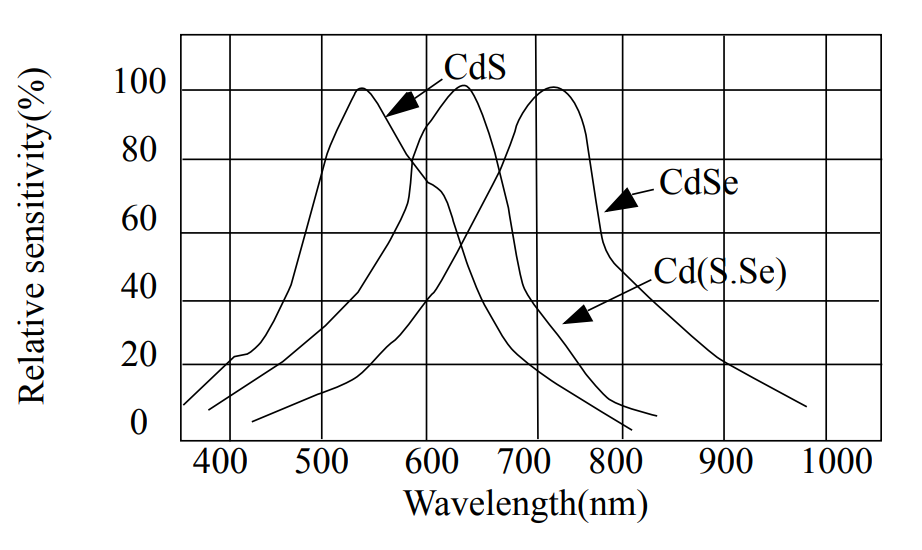
\includegraphics[width=\linewidth-0.1cm, keepaspectratio]{image2}
    \caption{CdS, CdSe ve Cd(S.Se) gibi Farklı Malzemelerin Spektral Yanıtları}
    \label{fig:spektralyanıt}
\end{figure}
\end{comment}


Projemizde kullandığımız iki LDR daha önce açıklandığı gibi MSP430 mikrodenetleyicisine bağlıdır. Bu LDR'lerden elde edilen gerilim sinyali MSP430 içindeki 12 bitlik SAR ADC kullanılarak dijital değerlere dönüştürülür.


\subsection{Ardışık Yaklaşım ADC}


\begin{figure}[H]
    \centering
    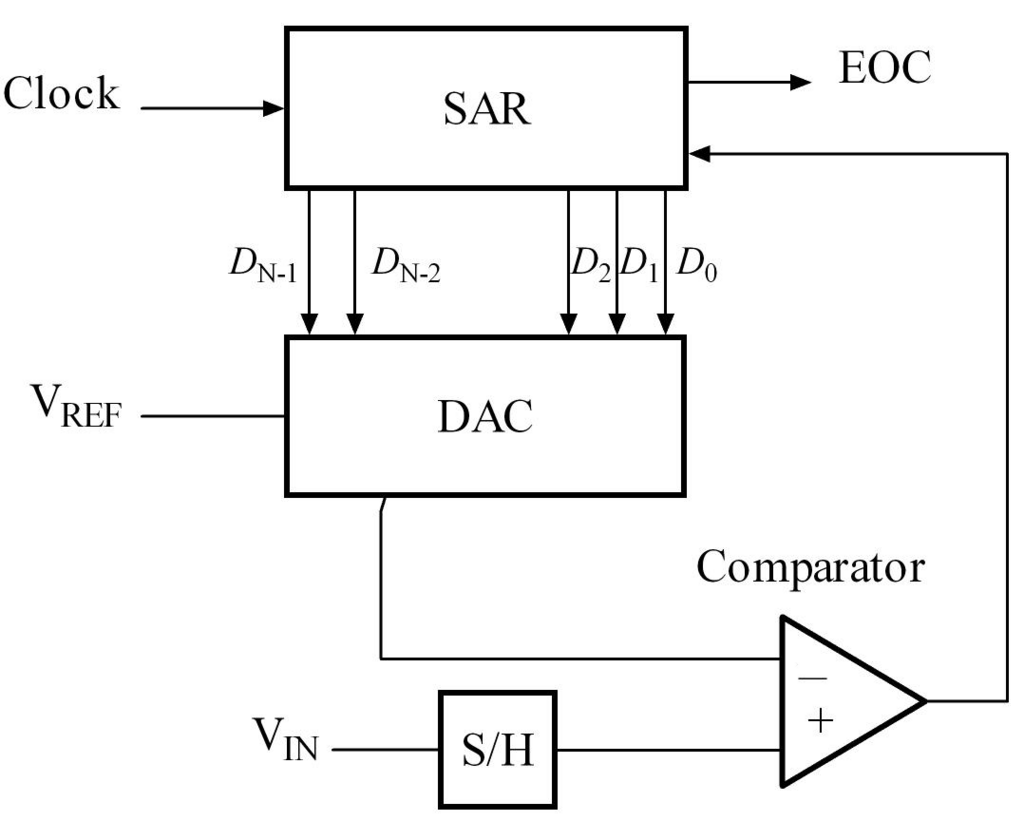
\includegraphics[width=0.75\linewidth]{image11.png}
    \caption{Ardışıl Yaklaşım ADC Diyagramı}
    \label{fig:sar-adc}
\end{figure}



\ref{fig:sar-adc}de Ardışık yaklaşım dönüştürücüsünün diyagramı verilmiştir. Ardışık yaklaşım dönüştürücüsü, nihai dijital cevaba ulaşmadan önce, tüm olası niceleme seviyeleri arasında ikili bir arama gerçekleştiren bir devredir. Devre $V_{in}$'i örnekler ve DAC'nin çıkışıyla karşılaştırır. Karşılaştırıcı çıkışı ikili aramanın yönünü kontrol eder ve ardışık yaklaşım kaydının (SAR) çıkışı asıl dijital dönüşümdür \cite{CMOS_SAR}. 

\newpage

Ardışık yaklaşım algoritması şu şekildedir:

\begin{tcolorbox}[colback=white, colframe=black, title={Ardışık Yaklaşım Algoritması}]
\begin{algorithmic}
\State Başlat: \(D_{N-1} \gets 1, D_{N-2} \gets 0, D_{N-3} \gets 0, \dots \gets D_0 \gets 0\)
\For{$i = N-1$ to $0$} (En anlamlı bitten başlayarak tüm bitler üzerinde yineleme yap)
    \State $V_{DAC} \gets D_{N-1} \cdot 2^{-1} + D_{N-2} \cdot 2^{-2} + \dots + D_{0} \cdot 2^{N-1}$
    \If{$V_{DAC} > V_{IN}$}
        \State \(D_i \gets 0\) olarak ayarla (\(V_{DAC} > V_{IN}\) ise biti sıfırla)
    \Else
        \State \(D_i \gets 1\) olarak bırak
    \EndIf
\EndFor
\State Sayısal değeri çıktı olarak ver : \(D = [D_{N-1}, D_{N-2}, \dots, D_0]\)
\end{algorithmic}
\end{tcolorbox}


Bu dijital veriler, daha önce açıklandığı gibi, sisteme entegre edilmiş olan HC05 Seri Bluetooth Modülü üzerinden aktarılır. Bu modül, verilerin kablosuz bir bağlantı aracılığıyla bilgisayara iletilmesini sağlar \cite{CMOS_SAR}. 


\subsection{HC05 Seri Bluetooth Modülü}

HC05 Seri Bluetooth modülü Bluetooth 2.0 + EDR versiyonunu kullanarak verileri aktarır. İlerleyen alt başlıklarda bu versiyon açıklanmıştır.

\subsubsection{Sistemin Yapısı}


Bluetooth'un ana sisteminin yapısı \ref{fig:bluetooth_core}da gösterilmiştir \cite{bluetooth2007core}. Mavi bağlantılar, protokol sinyallerini temsil ederken, siyah bağlantılar trafik taşıyıcıları üzerinden iletilmek üzere gönderilen sinyalleri ifade eder. Gri bağlantılar ise Bluetooth cihazının çalışma modunu, trafik taşıyıcılarını oluşturma, değiştirme ve serbest bırakma süreçlerini belirten sinyalleri gösterir. Sistem, her birinde kendine atanmış iletişim protokolü bulunan en alt 4 katmandan oluşmaktadır. Bazen bağlantı yöneticisi katmanı, temelbant katmanı ve radyo katmanı alt sistem olarak gruplandırılarak Bluetooth kontrolcüsü olarak adlandırılır. 


Kanal yöneticisi, uygulama verilerini ve servis protokollerini taşımak için kullanılan Mantıksal Bağlantı Kontrolü ve
Adaptasyon Protokolü (L2CAP) kanallarını oluşturma, yönetme ve sonlandırma işlemlerini gerçekleştirir \cite{bluetooth2007core}.

L2CAP kaynak yöneticisi Protokol Veri Birim (PDU) parçalarının temelbant'a gönderim sırasını yönetir ve Bluetooth kontrolcüsünün kaynak bitimi sebebiyle Protokol Kalitesi (QoS) taahhüdlü L2CAP kanallarının fiziksel kanallara erişiminin reddedilmemesini garanti etmek için kanallar arasındaki bazı alakalı zamanlamaları ayarlar \cite{bluetooth2007core}.


Cihaz yöneticisi Bluetooth cihazının genel davranışını kontrol eder. Veri iletimi ile alakalı olmayan bütün operasyonlardan sorumludur \cite{bluetooth2007core}.


Bağlantı yöneticisi Bağlantı Yönetimi Protokolü (LMP) kullanarak mantıksal bağlantılar oluşturmak ve değişiklik yapmakla sorumludur \cite{bluetooth2007core}.

\begin{figure}[H]
    \centering
    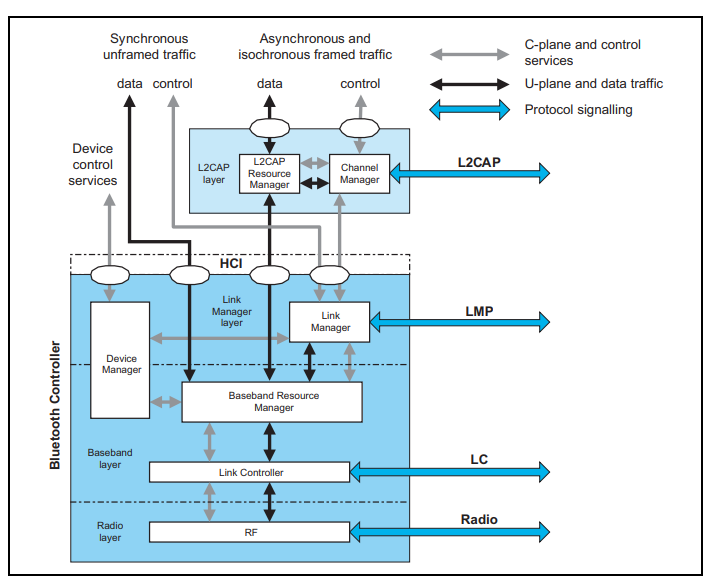
\includegraphics[width=\linewidth]{image21}
    \caption{Bluetooth Ana Sistemi}
    \label{fig:bluetooth_core}
\end{figure}



Temelbant kaynak yöneticisinin iki ana işlevi vardır. Temelinde, fiziksel kanallarda erişim sözleşmesi müzakere etmiş tüm birimlere zaman tanıyan bir zamanlayıcı bulunur. Diğer ana işlevi ise bu birimlerle erişim sözleşmeleri müzakere etmektir. Bir erişim sözleşmesi, bir kullanıcı uygulamasına beklenen bir performans sağlamak için gereken belirli bir QoS’yi sağlama taahhüdüdür \cite{bluetooth2007core}.


Bağlantı kontrolcüsü, Bluetooth paketlerinin fiziksel kanal, mantıksal taşıma ve mantıksal bağlantıyla ilgili veri yükü ve parametrelerinin kodlanması ve kodunun çözülmesinden sorumludur \cite{bluetooth2007core}.


Radyo Katmanı (RF) fiziksel kanaldaki paketlerin gönderimi ve alımından sorumludur \cite{bluetooth2007core}.


\subsubsection{Modülasyon Yöntemleri}

Modülasyon yöntemleri olarak Gaussian Frekans Kaymalı Anahtarlama (GFSK), $\pi/4$ döndürülmüş diferansiyel kodlamalı dörtlü faz kaydırmalı anahtarlama ($\pi/4$-DQPSK) ve diferansiyel kodlamalı sekizli faz kaydırmalı anahtarlama (8DPSK) kullanılır \cite{bluetooth2007core}.


\subsubsection{Taban Oran (BR)}

BR modunda bant genişliği zaman çarpımı (BT) 0.5 olan GFSK modülasyonu kullanılır. Modülasyon indeksi 0.28-0.35 arasıdır ve sembol zamanlaması $\pm20$ ppm den azdır. İkili 1 pozitif frekans ve ikili 0 negatif frekans kayması ile temsil edilir \cite{bluetooth2007core}.

\subsubsection{İkili Frekans Kaydırmalı Anahtarlama (BFSK)}

BFSK modülasyonu, taşıyıcı sinyalin $c(t)= \cos(2\pi f t)$ frekansını, gelen ikili veriye bağlı olarak iki farklı değere değiştiren bir yöntemdir. Verimizin fonksiyonu $d(t)$ olsun. O zaman modülasyon \eqref{eq:bfsk} daki gibidir \cite{BFSK}.

\begin{equation}
    y(t)=
    \begin{cases}
        \cos(2\pi (f_c+ f_d)t), & d(t)=1 \\
        \cos(2\pi( f_c+ f_d)t), &  d(t)=0 \\
    \end{cases}
    \label{eq:bfsk}
\end{equation}

\subsubsection{Gaussian Frekans Kaymalı Anahtarlama (GFSK)}

GFSK modülasyonu, veriyi önce Gaussian filtresi ile filtreler ve ardından 
Frekans Kaydırmalı Anahtarlama (FSK) modülasyonundan geçirir (Bluetooth için BFSK) \cite{bluetooth2007core}.

Gaussian filtresinin dürtü yanıtı \eqref{eq:gaussian} de gösterildiği gibidir \cite{gaussian}.

\begin{equation}
    g(x)= \sqrt{\frac{a}{\pi}}e^{-ax^2}
    \label{eq:gaussian}
\end{equation}


\subsubsection{Genişletilmiş Veri Oranı (EDR)}

EDR modunda kod ve paket başlığı verileri için BR GFSK; senkronizasyon dizisi, yük ve fragman dizisi için 2 Mbps $\pi/4$-DQPSK veya 3 Mbps 8DPSK modülasyonları kullanılır.

Modülasyon karekök yükseltilmiş kosinüs kullanarak veri sinyalini $v(t)$ oluşturur.
Vericinin çıktısı \eqref{eq:bluetooth_output} deki gibi temsil edilebilir \cite{bluetooth2007core}.

\begin{equation}
    S(t)=Re\left[v(t)e^{j\cdot 2\pi F_ct} \right]
    \label{eq:bluetooth_output}
\end{equation}

Bu modül ile bilgisayara gönderilen veriler Python kodu kullanılarak daha iyi analiz edilebilmesi için Üstel Hareketli Ortalama (EMA) filtresinden geçirilir.

\subsection{Üstel Hareketli Ortalama (EMA)}

EMA, üstel olarak azalan ağırlıklandırma faktörleri uygulayan birinci dereceden Sonsuz Dürtü Tepkisi (IIR) filtresidir. Veriler bu yöntem kullanılarak filtrelenir. Bu yöntem, verilerdeki ani dalgalanmaları düzeltir ve önemli değişiklikleri tespit etmeyi kolaylaştırır. IIR filtresinin genel matematiksel ifadesi aşağıdaki gibidir:

\begin{align}
 y[n] = & b_0 x[n] + b_1 x[n-1] + \cdots + b_P x[n-P] \label{eq:EMA} \\ 
      & + a_1 y[n-1] + a_2 y[n-2] - \cdots + a_Q y[n-Q] \nonumber
\end{align}


\eqref{eq:EMA} da P=0 ve Q=1 olursa birinci dereceden IIR filtre elde ederiz. Buna göre yeni \eqref{eq:EMA_real} şu şekilde olabilir.

\begin{equation}
    Y_t=\alpha X_t + (1-\alpha)Y_{t-1}
    \label{eq:EMA_real}
\end{equation}

Burada, \(\alpha\) filtreleme katsayısı, \(X_t\) şimdiki veri noktası, \(Y_t\) şimdiki filtrelenmiş veri noktası, \(Y_{t-1}\) bir önceki filtrelenmiş veri noktasıdır \cite{EMA}.

Filtrelenen veriler üzerinde geri yönde sonlu fark yöntemi uygulanarak birinin geçip geçmediği belirlenir.

\subsection{Geri Yönde Sonlu Fark}

Sonlu fark, $f(x+b) - f(x+a)$ biçimindeki matematiksel bir ifadedir. Geri yönde sonlu fark normal sonlu fark denkleminden farklı olarak $x + h$ ve $x$ değerleri yerine $x$ ve $x - h$'deki fonksiyon değerlerini kullanır:

\begin{equation}
    \nabla_h[f](x) = f(x) - f(x-h) = \Delta_h[f](x-h)
    \label{eq:finite_diff}
\end{equation}

\eqref{eq:finite_diff} de $\nabla$ fark operatörü olarak kullanılır. Fark operatörü f fonksiyonunu $\nabla f$ fonksiyonuna eşler \cite{FiniteDiff}.

Eğer bir geçiş tespit edilirse, bu kişiye ait veriler 500 sabit örnek içerecek şekilde düzenlenerek Virgülle Ayrılmış Değerler (CSV) formatında kaydedilir. Bu yöntem kullanılarak CSV dosyasına kaydedilen veriler MATLAB'e aktarılır. Bu veriler Z skoru normalizasyonu uygulandıktan sonra Gauss Gürültüsü eklenerek belirli sinyal gürültü oranı (SNR) değerlerinde veriler olacak şekilde eğitim veri seti oluşturmak için kullanılır.


\subsection{Z Skoru Normalizasyonu}
Z skoru normalizasyonu, bir verisetinde verisetinin ortalaması sıfır ve standart sapması bir olacak şekilde her bir veriyi normalize etme sürecine verilen isimdir.

Z skoru normalizasyonu yapılırken \eqref{eq:z1} deki formül her bir veriye uygulanır:

\begin{equation}
    z = \frac{(x - \mu)}{\sigma}
    \label{eq:z1}
\end{equation}

x: verinin orijinal değeri

$\mu$: verisetinin ortalama değeri

$\sigma$: verisetinin standart sapması

\begin{comment}
     E. Kreyszig (1979). Advanced Engineering Mathematics (Fourth ed.). Wiley. p. 880, eq. 5. ISBN 0-471-02140-7.
\end{comment}

\subsection{Gauss Gürültüsü}

Sinyal işleme teorisinde, Carl Friedrich Gauss'un adını taşıyan Gauss gürültüsü, olasılık yoğunluk fonksiyonu (PDF) normal dağılıma (Gauss dağılımı olarak da bilinir) eşit olan bir tür sinyal gürültüsüdür.

Derin öğrenme algoritmalarının eğitiminde modelin giriş verilerine gürültü eklemenin genelde çeşitli faydaları vardır:

Aşırı öğrenme olarak adlandırılan, modelin var olan veri kümesine fazla uyum göstermesi nedeniyle yeni veriler verildiğinde iyi tahminlerde bulunamama durumu azaltılabilir.

Gürültülü veri ile eğitilmiş modeller, yeni gelecek verileri daha iyi bir şekilde genelleyebilir.

\begin{comment}
    (Tudor Barbu (2013)Abstract and Applied Analysis. 2013: 8)
    (source:(Srivastava et al., 2014; Kingma
    et al., 2015; Poole et al., 2014))
\end{comment}



\subsection{Sinyal Gürültü Oranı}
Sinyal Gürültü Oranı (SNR), istenilen sinyal seviyesini arka plan gürültüsü seviyesine göre karşılaştıran bir ölçüdür. SNR, genellikle desibel (dB) cinsinden ifade edilen sinyal gücünün gürültü gücüne oranı olarak tanımlanır. 1:1'den büyük bir oran (0 dB'den büyük), sinyalin gürültüden daha fazla olduğunu gösterir. SNR, ayrıca belirli bir kanal üzerinden güvenilir bir şekilde iletilebilecek maksimum veri miktarını da belirler; bu, kanalın bant genişliğine ve SNR değerine bağlıdır. Bu ilişki, bilgi teorisinin temel yasalarından biri olan Shannon–Hartley teoremi ile açıklanır.

\begin{equation}
    \text{SNR} = \frac{P_{\text{signal}}}{P_{\text{noise}}},
    \label{eq:snr}
\end{equation}

Sinyal gürültü oranının ifadesi \eqref{eq:snr}'da verilmiştir.

\begin{comment}
    kaynak : Charles Sherman; John Butler (2007). Transducers and Arrays for Underwater Sound. Springer Science & Business Media. p. 276. ISBN 9780387331393.
\end{comment}


\subsection{Konvolüsyonel Gürültü Giderici Otokodlayıcı (CDAE)}

Bu çalışmada, gürültüden arındırılmış sinyalleri elde etmek için Konvolüsyonel Gürültü Giderici Otokodlayıcı (CDAE) kullanılmıştır. CDAE, temel olarak bir kodlayıcı, çözücü ve bu iki bölüm arasında yer alan gizli temsilden oluşur. Yapının derin öğrenme temelli olması, karmaşık örüntüleri öğrenmesine olanak tanımaktadır. CDAE, genel olarak Derin Sinir Ağları (Deep Neural Networks - DNN) ailesine ait bir yapıdır. DNN'ler, çok katmanlı yapıları sayesinde yüksek düzeyde soyut temsiller öğrenebilen yapay sinir ağlarıdır. CDAE, bu çerçevede özel olarak hem konvolüsyonel katmanlar (özellik çıkarımı için) hem de otokodlayıcı mimarisi (girdinin yeniden yapılandırılması için) kullanan bir türdür. Ayrıca, eğitim verisi gürültü giderici otokodlayıcı olarak yapılandırıldığı için, gürültülü girdilerden anlamlı temsiller öğrenerek orijinal sinyali yeniden üretme yeteneğine sahiptir. Bu özelliği sayesinde, hem temsil öğrenimi hem de sinyal temizleme amacıyla güçlü bir model sunar.


\subsubsection{Derin Sinir Ağları (DNN)}

DNN'ler, giriş ve çıkış katmanları arasında en az bir ara katman bulunan yapay sinir ağlarıdır. Bu ağlar, nöronlar, ağırlıklar, nöronlar arasındaki bağlantılar, eğilimler ve aktivasyon fonksiyonlarından oluşur. Her bir nöron, bir önceki katmandaki nöronlardan gelen bilgiyi (giriş katmanındaki nöronlar hariç) alır, bu bilgiyi ağırlıklarla sonraki katmandaki nöronlara aktarır (son katmandaki nöronlar hariç). Eğilimler, aktivasyon fonksiyonunun eşik değerini belirlerken, aktivasyon fonksiyonları yapay zekanın lineer olmayan ilişkileri öğrenmesini sağlar \cite{nielsen2015neural}.

Öncelikle, belirsizliği ortadan kaldırmak amacıyla bir DNN'in bileşenlerine ait notasyonların tanımlanması gerekmektedir.

\begin{itemize}
    \item $w^l_{jk}$: $(l-1)$'inci katmandaki $k$'ıncı nöron ile $l$'inci katmandaki $j$'inci nöron arasındaki bağlantının ağırlığı
    \item $w^l_j$: $(l-1)$'nci katmandaki nöronlar ile $l$'inci katmandaki $j$'inci nöron arasındaki bağlantıların ağırlıklarının vektörü
    \item $\hat{w}^l_j$ : $(l-1)$'nci katmandaki $j$'inci nöron ile $l$'inci katmandaki nöronlar arasındaki bağlantıların ağırlıklarının vektörü
    \item \( W^{l}\): katman \( l-1 \) ve katman \( l \) arasındaki ağırlıkları temsil eden bir matris. Burada matrisin elemanları \( w_{jk}^{l} \), katman \( l-1 \)'daki \( k \)-inci düğüm ile katman \( l \)'deki \( j \)-inci düğüm arasındaki ağırlığı temsil eder.
    \item $b^l_j$: $l$'inci katmandaki $j$'inci nöronun eğilimi (bias)
    \item $a^l_j$: $l$'inci katmandaki $j$'inci nöronun aktivasyonu
\end{itemize}


\ref{fig:DNN_exp}deki diyagramda, ağırlıklar, eğilimler ve aktivasyonlar gibi bileşenleri içeren örnek bir DNN yapısı, belirtilen notasyonlarla gösterilmiştir.


\begin{figure}[H]
    \centering
    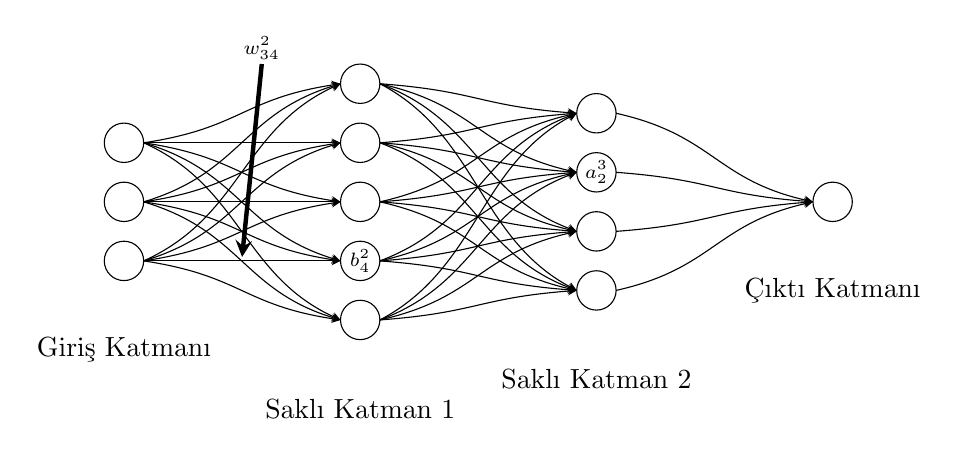
\begin{tikzpicture}[
    neuron/.style={circle, draw, minimum size=0.5cm, inner sep=0},
    arrow/.style={->, thick},
    align=center
    ]


    % Base coordinates
    \def\layers{3, 5, 4, 1} % Example: 3 input, 4 hidden, 3 hidden, 1 output
    \def\labels{Giriş Katmanı, Saklı Katman 1, Saklı Katman 2, Çıktı Katmanı}
    \def\features{}
    \def\xstart{0}    % X-coordinate for the first layer
    \def\layersep{3}  % Horizontal separation between layers
    \def\ysep{0.75}    % Vertical separation between neurons
    \def\maxneuron{11} % Threshold for number of neurons to display
    \pgfmathsetmacro{\mn}{int((\maxneuron-1)/2)}
    \pgfmathsetmacro{\ys}{int((\maxneuron+1)/2)}
    
    
    
    \foreach \i [count=\n from 1] in \layers {
        \ifnum\n = 1
            \foreach \feature [count=\n from 1] in \features {
                \pgfmathsetmacro{\yshift}{- (\i + 1) * \ysep / 2}
                \node[] at (-1.5, \yshift + \n*\ysep) {\feature};
            }
        \fi
    }
    
    
    % Process layers and neurons
    \foreach \i [count=\n from 1] in \layers {
        % Calculate the x-coordinate for the layer
        \pgfmathsetmacro{\xpos}{\xstart + (\n-1)*\layersep}
        
        % Draw neurons for the current layer and store node names in a list
        \ifnum\i > \maxneuron
            % Calculate vertical starting position for the neurons
            \pgfmathsetmacro{\yshift}{-\ys*\ysep}
            
            % Draw four neurons for the current layer
            \foreach \m in {1,2,...,\mn} {
                \pgfmathsetmacro{\t}{int(\maxneuron-\m)}
                \node[neuron] (L\n N\m) at (\xpos, \yshift + \m*\ysep) {};  % Node name L<layer> N<neuron>
                \node[neuron] (L\n N\t) at (\xpos, \m*\ysep) {};
            }
            % Add vertical ellipsis between second and third neuron
            \node at (\xpos, 0.125) {\huge$\vdots$};
        \else
            % Calculate vertical starting position for the neurons
            \pgfmathsetmacro{\yshift}{- (\i + 1) * \ysep / 2}
            
            
            % Draw all neurons for the current layer
            \foreach \m in {1,...,\i} {
                \node[neuron] (L\n N\m) at (\xpos, \yshift + \m*\ysep) {};  % Node name L<layer> N<neuron>
            }
        \fi
    }
    
    
    % Add layer labels
    \foreach \a [count=\m from 1] in \layers {
        \foreach \label [count=\n from 1] in \labels {
            \ifnum\n= \m
                \pgfmathsetmacro{\xpos}{(\n-1)*\layersep}
                \ifnum\a > \maxneuron
                    % Calculate vertical starting position for the neurons
                    \pgfmathsetmacro{\yshift}{-\maxneuron*\ysep/2}
                \else
                    % Calculate vertical starting position for the neurons
                    \pgfmathsetmacro{\yshift}{-\a*\ysep/2}
                \fi
                \node[align=center, font=\rmfamily] at (\xpos, \yshift - \ysep) {\label};
            \fi
        }
    }


    \draw[->, >=stealth, ultra thick] (\xstart + \layersep / 2 + 0.25, 2*\ysep + 0.25) -- (\xstart + 0.5*\layersep, -\ysep + 0.05);
    \node[font=\scriptsize] at (\xstart + \layersep / 2 + 0.25, 2*\ysep + 0.45) {$w^2_{34}$};
    \node[font=\scriptsize] at (\xstart + \layersep, -\ysep) {$b^2_{4}$};
    \node[font=\scriptsize] at (\xstart + 2*\layersep, \ysep/2) {$a^3_{2}$};
    
    
    % Loop through the list using pgffor
    \foreach \i [count=\n] in \layers {
        \foreach \j [count=\m] in \layers {
            \ifnum\m=\numexpr\n+1\relax
                \ifnum\i > \maxneuron
                    \pgfmathsetmacro{\ie}{\maxneuron-1}
                    \ifnum\j > \maxneuron
                        \pgfmathsetmacro{\je}{\maxneuron-1}
                        \foreach \k in {0,...,\ie} {
                            \foreach \p in {0,...,\je} {
                                \ifnum \numexpr2*\k = \ie 
                                \else
                                    \ifnum \numexpr2*\p = \je 
                                    \else
                                    \pgfmathsetmacro{\xpos}{\xstart + (\n-1)*\layersep}
                                    \pgfmathsetmacro{\yshift}{-\ys*\ysep}
                                    
                                    \pgfmathsetmacro{\nextlayer}{int(\n+1)}
                                    \draw[->, >=stealth] (\xpos + 0.25, \yshift + \k*\ysep + \ysep) .. controls (\xpos + \layersep / 2, \yshift + 3*\k*\ysep/4 + \p * \ysep / 4 + \ysep) and (\xpos + \layersep / 2, \yshift + 3*\p*\ysep / 4 + \k * \ysep / 4 + \ysep) .. (\xpos - 0.25 + \layersep, \yshift + \p*\ysep + \ysep);
                                    \fi
                                \fi
                            }
                        }
                    \else
                        \pgfmathsetmacro{\je}{\j}
                        \foreach \k in {0,...,\ie} {
                            \foreach \p in {1,...,\je} {
                                \ifnum \numexpr2*\k = \ie 
                                \else
                                \pgfmathsetmacro{\xpos}{\xstart + (\n-1)*\layersep}
                                \pgfmathsetmacro{\yshiftl}{- \ys * \ysep}
                                \pgfmathsetmacro{\yshiftr}{- (\je+1) * \ysep / 2}
                                
                                
                                \pgfmathsetmacro{\nextlayer}{int(\n+1)}
                                \draw[->, >=stealth] (\xpos + 0.25, \yshiftl + \k*\ysep + \ysep) .. controls (\xpos + \layersep / 2, 3*\yshiftl/4 + 3*\k*\ysep/4 + 3*\ysep/4 + \yshiftr/4 + \p*\ysep/4) and (\xpos + \layersep / 2, 3*\yshiftr/4 + 3*\p*\ysep/4 + \yshiftl/4 + \k*\ysep/4 + \ysep / 4) .. (\xpos - 0.25 + \layersep, \yshiftr + \p*\ysep);
                                \fi
                            }
                        }
                    \fi
                \else
                    \pgfmathsetmacro{\ie}{\i}
                    \ifnum\j > \maxneuron
                        \pgfmathsetmacro{\je}{\maxneuron-1}
                        \foreach \k in {1,...,\ie} {
                            \foreach \p in {0,...,\je} {
                                \ifnum \numexpr2*\p = \je 
                                \else
                                \pgfmathsetmacro{\xpos}{\xstart + (\n-1)*\layersep}
                                \pgfmathsetmacro{\yshiftl}{- (\ie + 1) * \ysep / 2}
                                \pgfmathsetmacro{\yshiftr}{-\ys * \ysep}
                                
                                
                                \pgfmathsetmacro{\nextlayer}{int(\n+1)}
                                \draw[->, >=stealth] (\xpos + 0.25, \yshiftl + \k*\ysep) .. controls (\xpos + \layersep / 2, 3*\yshiftl/4 + 3*\k*\ysep/4 + \yshiftr/4 + \p*\ysep/4 + \ysep/4) and (\xpos + \layersep / 2, 3*\yshiftr/4 + 3*\p*\ysep/4 + 3*\ysep/4 + \yshiftl/4 + \k*\ysep/4) .. (\xpos - 0.25 + \layersep, \yshiftr + \p*\ysep + \ysep);
                                \fi
                            }
                        }
                    \else
                        \pgfmathsetmacro{\je}{\j}
                        \foreach \k in {1,...,\ie} {
                            \foreach \p in {1,...,\je} {
                                \pgfmathsetmacro{\xpos}{\xstart + (\n-1)*\layersep}
                                \pgfmathsetmacro{\yshiftl}{- (\ie + 1) * \ysep / 2}
                                \pgfmathsetmacro{\yshiftr}{- (\je + 1) * \ysep / 2}
                                
                                \pgfmathsetmacro{\nextlayer}{int(\n+1)}
                                \draw[->, >=stealth] (\xpos + 0.25, \yshiftl + \k*\ysep) .. controls (\xpos + \layersep / 2, 3*\yshiftl/4 + 3*\k*\ysep/4 + \yshiftr/4 + \p*\ysep/4) and (\xpos + \layersep / 2, 3*\yshiftr/4 + 3*\p*\ysep/4 + \yshiftl/4 + \k*\ysep/4) .. (\xpos - 0.25 + \layersep, \yshiftr + \p*\ysep);
                            }
                        }
                    \fi
                \fi
            \fi
        }
    }
    
    
    \end{tikzpicture}
    \caption{Ağırlık, Eğilim ve Aktivasyon Bağlantılarını Vurgulayan Örnek Derin Sinir Ağı (DNN) Mimarisi}
    \label{fig:DNN_exp}
\end{figure}


\hyperref[fig:DNN_exp]{\protect\ref{fig:DNN_exp}}de, $w^2_{34}$, ikinci katmandaki dördüncü nöron ile üçüncü katmandaki ikinci nöron arasındaki bağlantının ağırlığını, $b^2_4$ ikinci katmandaki üçüncü nöronun eğilimini ve $a^3_2$ üçüncü katmandaki birinci nöronun aktivasyonunu ifade etmektedir.

Bunu daha iyi anlayabilmek için öncelikle nöronu tanımlayalım:

\begin{figure}
    \centering
    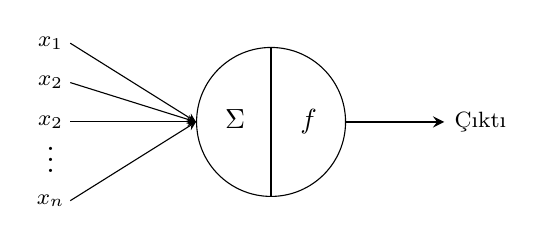
\begin{tikzpicture}[
    neuron/.style={circle, draw, minimum size=0.8cm, inner sep=0},
    input/.style={draw, -stealth},
    output/.style={draw, -stealth, thick},
    textnode/.style={align=center, font=\footnotesize}
    ]
    
    % Neuron node
    \node[neuron] (N) at (-0.2, 0) {$\hspace{1em} \Sigma \hspace{2em} f \hspace{1em}$};
    \draw[thick] (N.north) -- (N.south);
    
    % Input arrows
    \node[textnode] at (-3, 1) {$x_1$};
    \node[textnode] at (-3, 0.5) {$x_2$};
    \node[textnode] at (-3, 0) {$x_2$};
    \node at (-3, -0.375) {\large$\vdots$};
    \node[textnode] at (-3, -1) {$x_n$};
    
    \draw[input] (-2.75, 1) -- (N.west);
    \draw[input] (-2.75, 0.5) -- (N.west);
    \draw[input] (-2.75, 0) -- (N.west);
    \draw[input] (-2.75, -1) -- (N.west);
    
    
    % Output arrow
    \draw[output] (N.east) -- (2, 0) node[right, textnode] {Çıktı};
    
    \end{tikzpicture}
    \caption{Bir Nöronun Çalışma Şekli}
    \label{fig:nöron}
\end{figure}

\ref{fig:nöron}de de görüldüğü üzere bir nöronun $n\in\mathbb{N}$ adet girdi $(x_1, x_2,\dots,x_n)$ ve bir çıktısı vardır. Bu girdiler, giriş katmanından gelen verilerden veya diğer nöronların çıktılarından oluşabilir. Nöronun çıktısı, girdilerin belirli ağırlıklarla çarpılıp bir eğilim eklenerek elde edilen toplamın aktivasyon fonksiyonuna uygulanmasıyla bulunur. Matematiksel olarak bu, \eqref{eq:nöron-a} deki gibi ifade edilir \cite{nielsen2015neural}:

\begin{equation} 
    a^{l}_j = \sigma\left( \sum_k w^{l}_{jk} a^{l-1}_k + b^l_j\right)
    \label{eq:nöron-a}
\end{equation}


Teorik kısımda işlem basitliği sağlamak adına skaler çarpım işlemi $*$ operatörü ile tanımlanmıştır; yani, "x skaler çarpım y" işlemi $x * y \equiv \sum_i x_i y_i$ olarak ifade edilir. Bu tanımı kullanarak \eqref{eq:nöron-a} \eqref{eq:nöron-a-s1} e sadeleşir:
\begin{equation} 
    a^{l}_j = \sigma\left(w^l_j * a^{l-1}+b^l_j\right).
    \label{eq:nöron-a-s1}
\end{equation}

Son olarak bileşenleri $a^l_j$ aktivasyonları olan bir $a^l$ aktivasyon vektörü tanımlanır. Bu vektörü tanımlayabilmek için bir fonksiyonu özellikle aktivasyon fonksiyonunun vektörleştirilebilmesi lazım. Bir fonksiyonu vektörleştirmek, fonksiyona bir vektör verildiğinde, bu fonksiyonun vektördeki her bir bileşene ayrı ayrı uygulanması anlamına gelir. Bu tarz bir eleman yönlü (elementwise) işlemi göstermek için $\sigma(v)$ notasyonunu kullanılır (burada v, bir vektördür). Yani, $\sigma(v)$'nin bileşenleri $\sigma(v)_j = \sigma(v_j)$'dir.  Örnek olarak, mesela $f(x)=2\cdot x$ fonksiyonunun vektörleştirilmiş halinin $v=\left[ \begin{array}{c} 2 \\ 3 \end{array} \right]$ ye \eqref{eq:f_vector} de uygulandığı varsayılsın.
\begin{equation}
    f\left(\left[ \begin{array}{c} 2 \\ 3 \end{array} \right] \right)
        = \left[ \begin{array}{c} f(2) \\ f(3) \end{array} \right]
        = \left[ \begin{array}{c} 4 \\ 6 \end{array} \right]
        \label{eq:f_vector}
\end{equation}
Vektörleştirilmiş $f$ fonksiyonu her bir elemanın 2 katını almış olur. Bunu göz önünde bulundurarak \eqref{eq:nöron-a-s1} \eqref{eq:a^l} e değiştirilir:
\begin{equation}
    a^{l} = \sigma\left(W^l a^{l-1}+b^l\right)
    \label{eq:a^l}
\end{equation}
Ara bir değer olarak $z^l \equiv W^l a^{l-1} + b^l$ tanımlansın. Burada, $z^l_j$'nin bileşenlerinin $z^l_j \equiv w^l_j * a^{l-1} + b^l_j$ şeklindedir. Bu değer, maliyet fonksiyonunun gradyanını hesaplarken yararlı olacaktır.

Yani sonuç olarak sinir ağının son katmanının diğer bir deyişle çıktısının son hali \eqref{eq:a^l_z} deki gibi gösterilir:
\begin{equation} 
    a^{l} = \sigma(z^l)
    \label{eq:a^l_z}
\end{equation}

%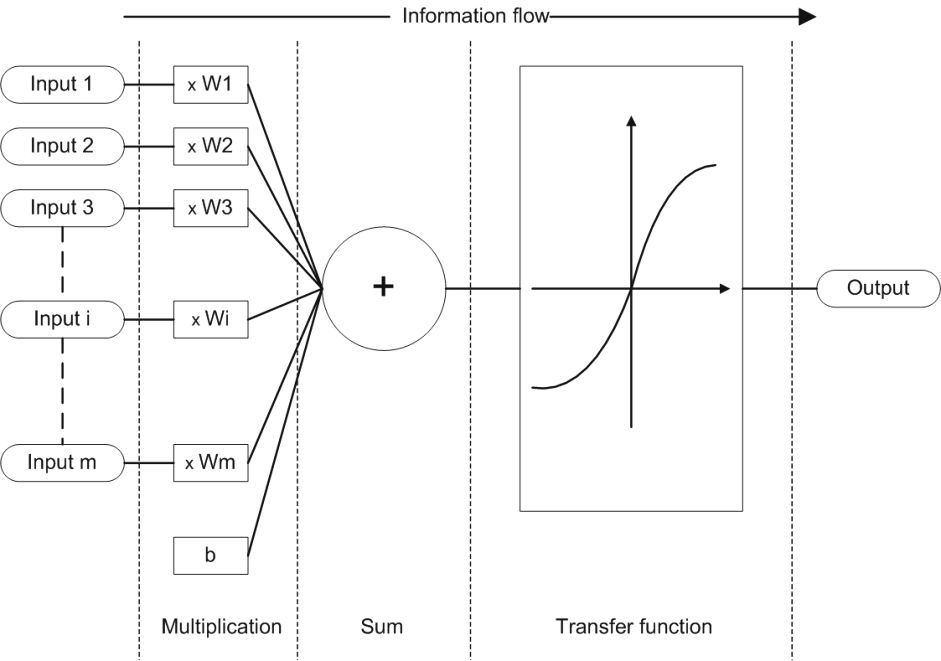
\includegraphics[width=\linewidth, keepaspectratio]{image8}
%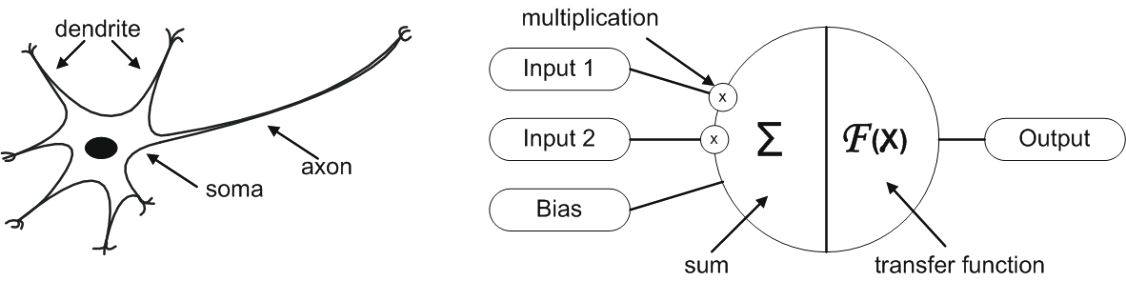
\includegraphics[width=\linewidth, keepaspectratio]{image9}

%\drawNN{3, 2, 1}{Input Layer, Hidden Layer, Output Layer}{Input 1, Input 2, Input 3}{2}{0.75}{11}

\subsubsection{CDAE Özellikleri}

DNN yapısının temel bileşenleri tanıtıldıktan sonra, bu yapının konvolüsyonel katmanlarla genişletilmiş hali olan CDAE mimarisi aşağıda açıklanmıştır.

Konvolüsyonel Gürültü Giderici Otokodlayıcı (CDAE) ağları, özellikle bozulmuş veya gürültülenmiş verilerin temiz halini yeniden oluşturmaya yönelik olarak tasarlanmış özel bir sinir ağı türüdür. Bu mimaride hem konvolüsyonel katmanlar hem de otokodlayıcı yapısı birlikte kullanılarak hem mekânsal özellikler korunur hem de sıkıştırma ve yeniden yapılandırma işlemleri gerçekleştirilir. Gürültü giderici otokodlayıcılar, giriş verisine yapay olarak eklenen bozulmaları öğrenerek bu bozulmaları telafi etmeyi amaçlar; böylece model, temel veri yapısını daha etkili bir biçimde öğrenir.

Özetle, klasik DNN'lar genel amaçlı öğrenme görevlerine yönelirken, CDAE'lar belirli bir görev olan gürültü azaltma ve girişin temiz halini yeniden oluşturma üzerine özelleşmiştir. Ayrıca, konvolüsyonel yapının dahil edilmesi, özellikle görüntü verilerinde, yerel bağıntıların ve mekânsal örüntülerin daha etkili biçimde yakalanmasını sağlar.


\subsection{Toplu Normalleştirme}

Toplu Normalleştirme, derin sinir ağlarının eğitimini iyileştirmek amacıyla her katmana gelen girdileri normalize eden bir tekniktir. Bu yöntem, her kanal için mini-toplu verisini tüm gözlemler boyunca normalize ederek çalışır; bu da eğitimi hızlandırır ve kararlılığı artırır.

Katman, aktivasyonları önce mevcut mini-toplu üzerinde hesaplanan ortalama çıkarılarak ve standart sapmaya bölünerek normalize eder. Bu işlem, eğitim sırasında katman girişlerinin dağılımının değişmesiyle ilgili olan içsel kovaryans kayması sorunlarını hafifletmeye yardımcı olur. Her bir giriş elemanı \( x_i \) için normalizasyon \eqref{eq:batch1} deki gibi tanımlanır:

\begin{equation}
    \widehat{x}_i = \frac{x_i - \mu_B}{\sqrt{\sigma_B^2 + \epsilon}},
    \label{eq:batch1}
\end{equation}

burada \( \mu_B \) ve \( \sigma_B^2 \), mini-toplu ortalaması ve varyansı olup, \( \epsilon \) ise sayısal kararlılık için eklenen küçük bir sabittir.

Normalizasyondan sonra, veriler öğrenilebilir parametrelerle dönüştürülerek ağın temsil gücü korunur:

\begin{equation}
    y_i = \gamma \widehat{x}_i + \beta,
    \label{eq:batch2}
\end{equation}

\eqref{eq:batch2} de \( \gamma \) öğrenilebilir bir ölçek parametresi ve \( \beta \) öğrenilebilir bir kaydırma parametresidir. Bu parametreler ağın diğer ağırlıklarıyla birlikte eğitilir.

Toplu Normalleştirme, ağ boyunca gradyanların akışını iyileştirerek optimizasyon yüzeyini daha düzgün hale getirir ve daha yüksek öğrenme oranlarının kullanılmasına olanak tanır. Ayrıca, bir örneğin aktivasyonları diğer örneklere bağlı olduğundan dolayı düzenleyici bir etki gösterir; bu da seyreltme veya güçlü ağırlık cezaları gibi diğer düzenleme tekniklerine olan ihtiyacı azaltabilir.

\begin{comment}
    https://www.mathworks.com/help/deeplearning/ref/nnet.cnn.layer.batchnormalizationlayer.html
\end{comment}


\subsection{Doğrultulmuş Doğrusal Ünite (ReLU)}


Yapay zeka bağlamında  Doğrultulmuş Doğrusal Ünite (Rectified Linear Unit – ReLU), bir aktivasyon fonksiyonudur. ReLU fonksiyonu, negatif giriş değerleri için sıfır, pozitif giriş değerleri için ise girişin kendisi kadar çıktı üretmektedir. Matematiksel olarak fonksiyon \eqref{eq:relu}'da tanımlanır \cite{zhang2014improving}. 


\begin{equation}
    f(x) = 
    \begin{cases}  
    x, & x > 0 \\  
    0, & x \leq 0  
    \end{cases}
    \label{eq:relu}
\end{equation}



\subsection{Geri Yayılım (Backpropagation)}

Geri yayılım algoritması incelenmeden önce maliyet fonksiyonu üzerinde durulması gerekmektedir. Maliyet fonksiyonunun, sinir ağının çıktılarının bir fonksiyonu olarak ifade edilebileceği varsayılmaktadır. \ref{fig:DNN_Cost} te bir maliyet fonksiyonu örneği sunulmaktadır. Bu varsayım, geri yayılım algoritmasının uygulanabilmesi için temel bir ön koşul oluşturmaktadır.

\begin{figure}[H]
    \centering
    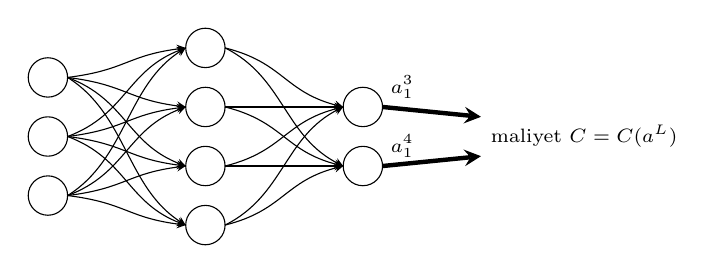
\begin{tikzpicture}[
    neuron/.style={circle, draw, minimum size=0.5cm, inner sep=0},
    arrow/.style={->, thick},
    align=center
    ]


    % Base coordinates
    \def\layers{3, 4, 2} % Example: 3 input, 4 hidden, 3 hidden, 1 output
    \def\labels{}
    \def\features{}
    \def\xstart{0}    % X-coordinate for the first layer
    \def\layersep{2}  % Horizontal separation between layers
    \def\ysep{0.75}    % Vertical separation between neurons
    \def\maxneuron{11} % Threshold for number of neurons to display
    \pgfmathsetmacro{\mn}{int((\maxneuron-1)/2)}
    \pgfmathsetmacro{\ys}{int((\maxneuron+1)/2)}
    
    
    
    \foreach \i [count=\n from 1] in \layers {
        \ifnum\n = 1
            \foreach \feature [count=\n from 1] in \features {
                \pgfmathsetmacro{\yshift}{- (\i + 1) * \ysep / 2}
                \node[] at (-1.5, \yshift + \n*\ysep) {\feature};
            }
        \fi
    }
    
    
    % Process layers and neurons
    \foreach \i [count=\n from 1] in \layers {
        % Calculate the x-coordinate for the layer
        \pgfmathsetmacro{\xpos}{\xstart + (\n-1)*\layersep}
        
        % Draw neurons for the current layer and store node names in a list
        \ifnum\i > \maxneuron
            % Calculate vertical starting position for the neurons
            \pgfmathsetmacro{\yshift}{-\ys*\ysep}
            
            % Draw four neurons for the current layer
            \foreach \m in {1,2,...,\mn} {
                \pgfmathsetmacro{\t}{int(\maxneuron-\m)}
                \node[neuron] (L\n N\m) at (\xpos, \yshift + \m*\ysep) {};  % Node name L<layer> N<neuron>
                \node[neuron] (L\n N\t) at (\xpos, \m*\ysep) {};
            }
            % Add vertical ellipsis between second and third neuron
            \node at (\xpos, 0.125) {\huge$\vdots$};
        \else
            % Calculate vertical starting position for the neurons
            \pgfmathsetmacro{\yshift}{- (\i + 1) * \ysep / 2}
            
            
            % Draw all neurons for the current layer
            \foreach \m in {1,...,\i} {
                \node[neuron] (L\n N\m) at (\xpos, \yshift + \m*\ysep) {};  % Node name L<layer> N<neuron>
            }
        \fi
    }
    
    
    % Add layer labels
    \foreach \a [count=\m from 1] in \layers {
        \foreach \label [count=\n from 1] in \labels {
            \ifnum\n= \m
                \pgfmathsetmacro{\xpos}{(\n-1)*\layersep}
                \ifnum\a > \maxneuron
                    % Calculate vertical starting position for the neurons
                    \pgfmathsetmacro{\yshift}{-\maxneuron*\ysep/2}
                \else
                    % Calculate vertical starting position for the neurons
                    \pgfmathsetmacro{\yshift}{-\a*\ysep/2}
                \fi
                \node[align=center, font=\rmfamily] at (\xpos, \yshift - \ysep) {\label};
            \fi
        }
    }


    \draw[->, >=stealth, ultra thick] (\xstart + 2*\layersep + 0.25, \ysep / 2) -- (\xstart + 2*\layersep + 1.5, \ysep/2 - 0.125);
    \draw[->, >=stealth, ultra thick] (\xstart + 2*\layersep + 0.25, -\ysep / 2) -- (\xstart + 2*\layersep + 1.5, -\ysep/2 + 0.125);
    
    \node[font=\scriptsize] at (\xstart + 2*\layersep + \ysep/2 + 0.125, \ysep/2 + 0.25) {$a^3_{1}$};
    \node[font=\scriptsize] at (\xstart + 2*\layersep + \ysep/2 + 0.125, -\ysep/2 + 0.25) {$a^4_{1}$};
    \node[font=\scriptsize, anchor=west] at (\xstart + 2*\layersep + 1.5, 0) {maliyet $C = C(a^L)$};
    
    
    % Loop through the list using pgffor
    \foreach \i [count=\n] in \layers {
        \foreach \j [count=\m] in \layers {
            \ifnum\m=\numexpr\n+1\relax
                \ifnum\i > \maxneuron
                    \pgfmathsetmacro{\ie}{\maxneuron-1}
                    \ifnum\j > \maxneuron
                        \pgfmathsetmacro{\je}{\maxneuron-1}
                        \foreach \k in {0,...,\ie} {
                            \foreach \p in {0,...,\je} {
                                \ifnum \numexpr2*\k = \ie 
                                \else
                                    \ifnum \numexpr2*\p = \je 
                                    \else
                                    \pgfmathsetmacro{\xpos}{\xstart + (\n-1)*\layersep}
                                    \pgfmathsetmacro{\yshift}{-\ys*\ysep}
                                    
                                    \pgfmathsetmacro{\nextlayer}{int(\n+1)}
                                    \draw[->, >=stealth] (\xpos + 0.25, \yshift + \k*\ysep + \ysep) .. controls (\xpos + \layersep / 2, \yshift + 3*\k*\ysep/4 + \p * \ysep / 4 + \ysep) and (\xpos + \layersep / 2, \yshift + 3*\p*\ysep / 4 + \k * \ysep / 4 + \ysep) .. (\xpos - 0.25 + \layersep, \yshift + \p*\ysep + \ysep);
                                    \fi
                                \fi
                            }
                        }
                    \else
                        \pgfmathsetmacro{\je}{\j}
                        \foreach \k in {0,...,\ie} {
                            \foreach \p in {1,...,\je} {
                                \ifnum \numexpr2*\k = \ie 
                                \else
                                \pgfmathsetmacro{\xpos}{\xstart + (\n-1)*\layersep}
                                \pgfmathsetmacro{\yshiftl}{- \ys * \ysep}
                                \pgfmathsetmacro{\yshiftr}{- (\je+1) * \ysep / 2}
                                
                                
                                \pgfmathsetmacro{\nextlayer}{int(\n+1)}
                                \draw[->, >=stealth] (\xpos + 0.25, \yshiftl + \k*\ysep + \ysep) .. controls (\xpos + \layersep / 2, 3*\yshiftl/4 + 3*\k*\ysep/4 + 3*\ysep/4 + \yshiftr/4 + \p*\ysep/4) and (\xpos + \layersep / 2, 3*\yshiftr/4 + 3*\p*\ysep/4 + \yshiftl/4 + \k*\ysep/4 + \ysep / 4) .. (\xpos - 0.25 + \layersep, \yshiftr + \p*\ysep);
                                \fi
                            }
                        }
                    \fi
                \else
                    \pgfmathsetmacro{\ie}{\i}
                    \ifnum\j > \maxneuron
                        \pgfmathsetmacro{\je}{\maxneuron-1}
                        \foreach \k in {1,...,\ie} {
                            \foreach \p in {0,...,\je} {
                                \ifnum \numexpr2*\p = \je 
                                \else
                                \pgfmathsetmacro{\xpos}{\xstart + (\n-1)*\layersep}
                                \pgfmathsetmacro{\yshiftl}{- (\ie + 1) * \ysep / 2}
                                \pgfmathsetmacro{\yshiftr}{-\ys * \ysep}
                                
                                
                                \pgfmathsetmacro{\nextlayer}{int(\n+1)}
                                \draw[->, >=stealth] (\xpos + 0.25, \yshiftl + \k*\ysep) .. controls (\xpos + \layersep / 2, 3*\yshiftl/4 + 3*\k*\ysep/4 + \yshiftr/4 + \p*\ysep/4 + \ysep/4) and (\xpos + \layersep / 2, 3*\yshiftr/4 + 3*\p*\ysep/4 + 3*\ysep/4 + \yshiftl/4 + \k*\ysep/4) .. (\xpos - 0.25 + \layersep, \yshiftr + \p*\ysep + \ysep);
                                \fi
                            }
                        }
                    \else
                        \pgfmathsetmacro{\je}{\j}
                        \foreach \k in {1,...,\ie} {
                            \foreach \p in {1,...,\je} {
                                \pgfmathsetmacro{\xpos}{\xstart + (\n-1)*\layersep}
                                \pgfmathsetmacro{\yshiftl}{- (\ie + 1) * \ysep / 2}
                                \pgfmathsetmacro{\yshiftr}{- (\je + 1) * \ysep / 2}
                                
                                \pgfmathsetmacro{\nextlayer}{int(\n+1)}
                                \draw[->, >=stealth] (\xpos + 0.25, \yshiftl + \k*\ysep) .. controls (\xpos + \layersep / 2, 3*\yshiftl/4 + 3*\k*\ysep/4 + \yshiftr/4 + \p*\ysep/4) and (\xpos + \layersep / 2, 3*\yshiftr/4 + 3*\p*\ysep/4 + \yshiftl/4 + \k*\ysep/4) .. (\xpos - 0.25 + \layersep, \yshiftr + \p*\ysep);
                            }
                        }
                    \fi
                \fi
            \fi
        }
    }
    
    
    \end{tikzpicture}
    \caption{Maliyet Fonksiyonu}
    \label{fig:DNN_Cost}
\end{figure}

İkinci dereceden maliyet fonksiyonu bu şartı sağlar, çünkü maliyet fonksiyonu \eqref{eq:cost_example} deki gibi ifade edilebilir. \begin{equation} C = \frac{1}{2} |y-a^L|^2 = \frac{1}{2} \sum_j (y_j-a^L_j)^2 \label{eq:cost_example} \end{equation} Bu durumda, maliyet fonksiyonu ağın çıktılarının bir fonksiyonu olarak yazılabilir. Bu tür bir maliyet fonksiyonu, ağın ağırlıklarının güncellenmesi için gerekli olan gradyanların hesaplanmasını mümkün kılar. Geri yayılım algoritması, gradyanları vektör toplama, bir vektörü bir matrisle çarpma gibi temel lineer cebir operatörleri kullanarak hesaplar. Ancak, bu operatörlerden biri daha nadir olarak kullanılır; bu operatör Hadamard Çarpımı'dır \cite{nielsen2015neural}.

\subsubsection{Hadamard Çarpımı \(\mathbf{\left( s \odot t \right)}\)}

Varsayalım ki s ve t aynı boyuta sahip iki vektör. O zaman bu iki vektörün eleman yönlü çarpımını göstermek için $s \odot t$ kullanılır. Burada, $s \odot t$ nin bileşenleri $\left(s \odot t\right)_j=s_jt_j$ şeklinde tanımlanır. Bu tezde, bu çarpma işlemi için Hadamard çarpımı terimi kullanılacaktır \cite{nielsen2015neural}.

\subsubsection{Geri Yayılımdaki Dört Temel Denklem}

Geri yayılım, bir ağdaki ağırlıkları ve eğilimleri değiştirmek için maliyet fonksiyonunun gradyanını kullanır. İlk olarak hata $\delta^l_j$ tanımlanır.

Hata $\delta^l_j$ \eqref{eq:error} deki gibi ifade edilir.
\begin{equation}
    \delta^l_j \equiv \frac{\partial C}{\partial z^l_j}
    \label{eq:error}
\end{equation}

\eqref{eq:error} zincir kuralı kullanılarak şu şekilde yazılabilir:
\begin{equation}
    \begin{split}
        \delta^L_j = \frac{\partial C}{\partial z^L_j} &= \frac{\partial C}{\partial a^L_j}\frac{\partial a^L_j}{\partial z^L_j} \\ &= \frac{\partial C}{\partial a^L_j}\frac{\partial \sigma}{\partial z^L_j} \left( z^L_j \right) \\ &= \frac{\partial C}{\partial a^L_j} \sigma'(z^L_j)
    \end{split}
    \label{eq:error-s}
\end{equation}

\eqref{eq:error-s} hata $\delta^L$ için eleman yönlü bir ifadedir. Fakat geri yayılım için matris formundaki hali lazımdır. \eqref{eq:error-s} i tekrar matris formunda yazarsak:
\begin{equation}
    \delta^L = \nabla_a C \odot \sigma'(z^L)
    \label{eq:error-v}
\end{equation}
\eqref{eq:error-v} de $\nabla_a C$ bileşenleri kısmi türevler $\partial C / \partial a^L_j$ olan bir vektördür.
Bu hata $\delta^l$ yi bir sonraki katmana göre hesaplanabilir.
\begin{equation}
    \delta^l = \left((W^{l+1})^T \delta^{l+1} \right) \odot \sigma'(z^l)
    \label{eq:error-r}
\end{equation}


\eqref{eq:error-r} de $(W^{l+1})^T$ $(l+1)$'nci katmanın ağırlık matrisinin devriğidir.
\eqref{eq:error-v-p} aşağıdaki şekilde çıkarılabilir:
\begin{equation}
    \begin{split}
        \delta^l_j &= \frac{\partial C}{\partial z^l_j} \\
                                &= \sum_k \frac{\partial C}{\partial z^{l+1}_k} \frac{\partial z^{l+1}_k}{\partial z^l_j} \\ 
                                &= \sum_k \delta^{l+1}_k \frac{\partial}{\partial z^l_j}  \left( \sum_i w^{l+1}_{ki} \sigma(z^l_i) +b^{l+1}_k \right) \\
                                &= \sum_k w^{l+1}_{kj}  \delta^{l+1}_k \sigma'(z^l_j) \\
                                &= \left( \hat{w}^{l+1}_j * \delta^{l+1} \right)_j \sigma'(z^l_j) \\
                                &=  (W^{l+1})^T \delta^{l+1} \odot \sigma'(z^l_j)
    \end{split}
    \label{eq:error-v-p}
\end{equation}

\eqref{eq:error-v} ile \eqref{eq:error-r} i birleştirerek, ağdaki herhangi bir katman için hata $\delta^l$'i hesaplanabilir.

Artık maliyet fonksiyonunun herhangi bir ağırlığa veya yanlılığa göre gradyanı hesaplanabilir. Maliyet fonksiyonunun gradyanı herhangi bir ağırlığa veya yanlılığa göre \eqref{eq:weight_bias} deki gibi hesaplanır \cite{nielsen2015neural}. 

\begin{equation}
    \label{eq:weight_bias}
    \begin{split}
        \frac{\partial C}{\partial w^l_{jk}} &= \frac{\partial C}{\partial z^l_j}\frac{\partial z^l_j}{\partial w^l_{jk}} \\ 
        &= \delta^l_j \frac{\partial}{\partial w^l_{jk}}\left( \sum_i w^l_{ji}a^{l-1}_i + b^l_i \right) \\ 
        &= \delta^l_j a^{l-1}_k
    \end{split}
    \qquad
    \begin{split}
        \frac{\partial C}{\partial b^l_j} &=  \frac{\partial C}{\partial z^l_j}\frac{\partial z^l_j}{\partial b^l_j} \\ 
        &= \delta^l_j \frac{\partial}{\partial b^l_j}\left( w^l_j * a^{l-1}_j + b^l_j \right) \\ 
        &= \delta^l_j
    \end{split}
\end{equation}



\begin{table}[H]
\centering
\renewcommand{\arraystretch}{2}
\begin{tabular}{|lr|}
\hline
\multicolumn{2}{|c|}{\textbf{Özet: Geri Yayılım Denklemleri}} \\
$\delta^L = \nabla_a C \odot \sigma^{\prime}\left(z^L\right)$ & \eqref{eq:error-v}\\
$\delta^l = \left( \left(W^{l+1}\right)^T \delta^{l+1} \right) \odot \sigma^{\prime}\left(z^l\right)$ & \eqref{eq:error-r} \\
$\frac{\partial C}{\partial b_j^l} = \delta_j^l$ & \eqref{eq:weight_bias} \\
$\frac{\partial C}{\partial w_{jk}^l} = a_k^{l-1} \delta_j^l$ & \eqref{eq:weight_bias} \\
\hline
\end{tabular}
\end{table}

\subsubsection{Geri Yayılım Algoritması}

Geri yayılım algoritması aşağıdaki gibidir:

\begin{itemize}
    \item \textbf{Girdi x:} Giriş katmanına karşılık gelen aktivasyon $a^1$ i tanımlanır.
    \item \textbf{İleri Besleme:} Her $l = 2, 3, \ldots, L$ için $z^l=w^la^{l-1}+b^l$ ve $a^l=\sigma(z^l)$ hesaplanır.
    \item \textbf{Çıktı Hatası $\delta^L$:} $\delta^{L} = \nabla_a C \odot \sigma'(z^L)$ vektörü hesaplanır.
    \item \textbf{Hatayı geri yay:} Her $l=L-1,L-2,\ldots,2$ için $\delta^l=((W^{l+1})^T \delta^{l+1}) \odot \sigma'(z^{l})$ hesaplanır.
    \item \textbf{Çıktı:} Maliyet fonksiyonunun gradyanı $\frac{\partial C}{\partial w^l_{jk}} = a^{l-1}_k \delta^l_j$ ve $\frac{\partial C}{\partial b^l_j} = \delta^l_j$ ile bulunmuş olur \cite{nielsen2015neural}.
\end{itemize}

\subsection{Rastgele Gradyan İnişi (SGD)}

Rastgele gradyan inişinde, gerçek gradyanı, tek bir örnekteki gradyan ile yaklaşık olarak hesaplanır ve her $l = L, L-1, \ldots, 2$ için ağırlıklar $w^l \rightarrow w^l-\eta \cdot \delta^l (a^{l-1})^T$ kuralına göre ve eğilimler $b^l \rightarrow b^l-\eta \cdot \delta^l$ kuralına göre güncellenir \cite{StochasticLeon}.


\subsection{Adam optimize edici}

Adam (Adaptive Moment Estimation), rastgele gradyan inişi (SGD) yönteminin bir çeşididir. Yöntem, gradyanların birinci ve ikinci momentlerinin kestirimlerinden farklı parametreler için bireysel uyarlanabilir öğrenme oranlarını hesaplar.

\textbf{Algoritma:}

Algoritma, gradyanın (\(m_t\)) ve kareli gradyanın (\(v_t\)) üssel hareketli ortalamalarını günceller. Burada \(\beta_1, \beta_2 \in [0, 1)\) hiperparametreleri bu değerlerin üstel azalma oranlarını belirler. Hareketli ortalamalar, gradyanın 1. anının (ortalama) ve 2. ham anının (merkezlenmemiş varyans) kestirimleridir.


Algoritmanın işleyişi aşağıda detaylı olarak adım adım açıklanmıştır:
\begin{enumerate}
    \item \textbf{Başlatma:}
    \begin{itemize}
        \item $m_0 \gets 0$: 1. moment vektörü (ortalama) sıfırla başlatılır.
        \item $v_0 \gets 0$: 2. moment vektörü (varyans) sıfırla başlatılır.
        \item $t \gets 0$: Zaman adımı 0 olarak ayarlanır.
    \end{itemize}
    
    \item \textbf{Döngü:} Algoritma, parametre $\theta_t$ yakınsamaya ulaşana kadar şu adımları tekrarlar:
    \begin{enumerate}
        \item \textbf{Gradyan Hesaplama:}
        \begin{equation}
        g_t \gets \nabla_\theta f_t(\theta_{t-1})
        \label{eq:gt}
        \end{equation}
        \eqref{eq:gt} de $t$ adımındaki stokastik hedef fonksiyonun gradyanı hesaplanır.
        
        \item \textbf{1. Moment Güncelleme:}
        \begin{equation}
        m_t \gets \beta_1 \cdot m_{t-1} + (1 - \beta_1) \cdot g_t
        \label{eq:mt}
        \end{equation}
        \eqref{eq:mt} önceki moment ($m_{t-1}$) ile yeni gradyanı ($g_t$) birleştirerek hareketli bir ortalama oluşturur.
        
        \item \textbf{2. Moment Güncelleme:}
        \begin{equation}
        v_t \gets \beta_2 \cdot v_{t-1} + (1 - \beta_2) \cdot g_t^2
        \label{eq:vt}
        \end{equation}
        \eqref{eq:vt} gradyanın karesini alarak değişkenlik (varyans) kestirimi yapar.
        
        \item \textbf{Eğilim Düzeltilmesi:}
        \begin{itemize}
            \item 1. moment için:
            \begin{equation}
            \hat{m}_t \gets \frac{m_t}{1 - \beta_1^t}
            \label{eq:mt_h}
            \end{equation}
            \eqref{eq:mt_h} moment kestirmesinin başlangıçtaki sıfır durumundan kaynaklanan eğilimi giderir.
            \item 2. moment için:
            \begin{equation}
            \hat{v}_t \gets \frac{v_t}{1 - \beta_2^t}
            \label{eq:vt_h}
            \end{equation}
            Benzer şekilde \eqref{eq:vt_h} de, 2. moment kestirmesi düzeltilir.
        \end{itemize}
        
        \item \textbf{Parametre Güncelleme:}
        \begin{equation}
        \theta_t \gets \theta_{t-1} - \alpha \cdot \frac{\hat{m}_t}{\sqrt{\hat{v}_t} + \epsilon}
        \label{eq:theta_t}
        \end{equation}
        \eqref{eq:theta_t} de $\epsilon$, sıfıra bölme hatasını önlemek için kullanılan küçük bir sabittir (örneğin, $10^{-8}$).
    \end{enumerate}
    
    \item \textbf{Sonuç:} Algoritma, yakınsama sağlandığında $\theta_t$ değerini döndürür \cite{kingma2017adammethodstochasticoptimization}.
\end{enumerate}


Algoritması, sözde kod olarak, \cite{kingma2017adammethodstochasticoptimization} makalesinden alınmıştır ve \ref{fig:adamalg}'de gösterildiği şekilde bulunabilir.

\subsubsection{L2 Düzenlemesi}

Ağırlıklar için $E(\theta)$ kayıp fonksiyonuna bir düzenleme terimi ekleyerek, aşırı öğrenmeyi azaltır \cite{PaterrecogBishop, machinelearning:2012}. Düzenleme terimine ağırlık azalması da denir. Düzenleme terimine sahip kayıp fonksiyonu \eqref{eq:L2} deki gibidir:

\begin{equation}
    E_R(\theta)=E(\theta)+\lambda \Omega(w)
    \label{eq:L2}
\end{equation}

\eqref{eq:L2} de $w$ ağırlık vektörüdür, $\lambda$ düzenleme faktörüdür (katsayı) ve düzenleme fonksiyonu $\Omega(w)$ \eqref{eq:düzenleme} deki gibidir:

\begin{equation}
    \Omega(w)=\frac{1}{2} w^T w
    \label{eq:düzenleme}
\end{equation}

Eğilimler düzenlenmez \cite{machinelearning:2012}.

\begin{figure}[H]
    \centering
    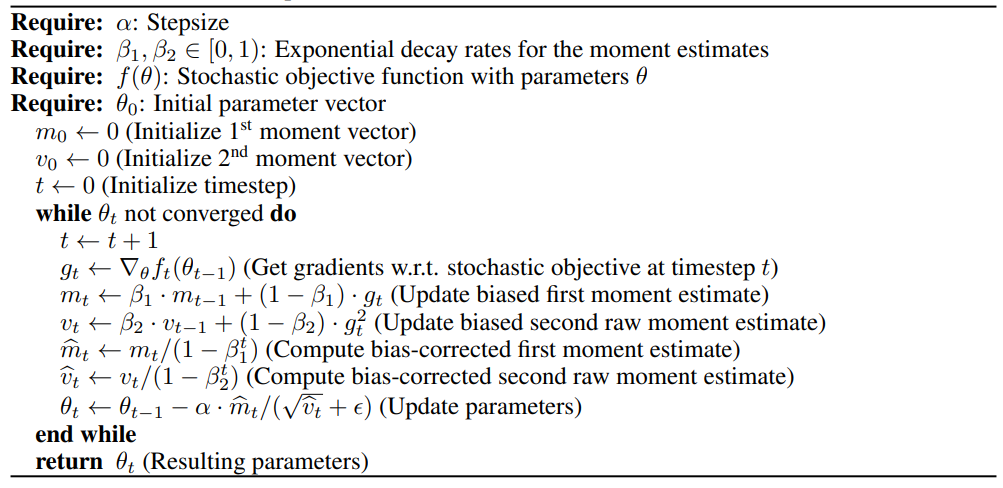
\includegraphics[width=\linewidth]{image17}
    \caption{Adam Algoritması Sözde Kodu}
    \label{fig:adamalg}
\end{figure}

\subsubsection{Gradyan Kırpma}

Gradyanların büyüklükleri üssel olarak artarsa, eğitim kararsızlaşır ve birkaç yineleme içinde farklılaşabilir. Bu "gradyan patlaması", NaN veya Inf'e giden bir eğitim kaybı demektir. Gradyan kırpma, eğitimi daha yüksek öğrenme oranlarında ve aykırı değerlerin olduğu durumlarda sabitleyerek gradyan patlamasını önlemeye yardımcı olur \cite{trainrecneural}. Gradyan kırpma, ağların daha hızlı eğitilmesini sağlar ve genellikle öğrenilen görevin doğruluğunu etkilemez.

İki tür gradyan kırpma vardır.
\begin{itemize}
\item Vektör büyüklüğü tabanlı gradyan kırpma, gradyanı bir eşik değerine göre yeniden ölçeklendirir ve gradyanın yönünü değiştirmez.
\item Değer tabanlı gradyan kırpma, eşikten büyük olan herhangi bir kısmi türevi keser ve bu da gradyanın keyfi olarak yön değiştirmesine neden olabilir. Değer tabanlı gradyan kırpma öngörülemeyen bir davranışa sahip olabilir, ancak yeterince küçük değişiklikler ağın ıraksamasına neden olmaz.
\end{itemize}

\begin{comment}
2. Text 2 ile Karşılaştırma: Eksik, Yarım veya Var mı?
Kısım	Text 2’de Anlatım Durumu	Açıklama / Önerilen Başlıklar
Veri Girişi ve Yapısı	Yarım veya eksik	Model giriş verisinin iki LDR’den 500’er ölçüm olarak birleştirildiği net değil. Burada mutlaka "Veri Seti ve Ön İşleme" başlığı altında açıklanmalı. Özellikle 1000 boyutlu vektör yapısı detaylandırılmalı.
Z-score Normalizasyon	Muhtemelen yok veya yetersiz	Veri normalizasyonun neden gerekli olduğu ve nasıl yapıldığı anlatılmalı. "Veri Ön İşleme" altında yer almalı.
Veri Bölme (Train-Val)	Yarım veya muhtemelen eksik	Veri bölme ve validasyon stratejisi net açıklanmalı. "Veri Seti Hazırlığı" veya "Model Eğitimi İçin Veri Hazırlığı" altında işlenmeli.
Veri Artırma (augmentData)	Büyük ihtimalle yok	Özellikle SNR tabanlı gürültü eklenmesi detaylandırılmalı, gerekçeleri anlatılmalı. "Veri Artırma ve Gürültü Modellenmesi" başlığı açılabilir.
Model Mimarisi (Autoencoder)	Yarım veya eksik	Text 2’de klasik DNN varken Text 3’de konvolüsyonel denoising autoencoder var. Bu önemli değişiklik "Model Mimarisi" başlığı altında açık ve detaylı anlatılmalı. Katmanlar, kernel boyutları, dropout, batch norm gibi teknik detaylar burada yer almalı.
Eğitim Parametreleri ve Metodoloji	Yarım veya eksik	Öğrenme hızı, epoch sayısı, erken durdurma, optimizasyon ayarları vb. ayrıntılı şekilde "Model Eğitimi" başlığı altında yer almalı.
Rekonstrüksiyon Hatası ve Eşik Belirleme	Eksik veya yok	Model çıktılarının değerlendirilmesi, hata hesaplaması, eşik belirleme metodolojisi "Model Değerlendirmesi" başlığında yer almalı.
Embedding Çıkarımı ve Kümeleme	Muhtemelen yok veya eksik	Özellikle "Anomali Tespiti İçin Özellik Çıkarımı ve Kümeleme" gibi bir başlık açılarak embedding çıkarmanın mantığı, k-means uygulaması, etiket eşleştirme detaylandırılmalı.
Hungarian Algoritması ile Etiket Eşleme	Büyük ihtimalle yok	Karmaşık kümeleme sonrası etiket eşleştirme yöntemi yeni ve önemli, ayrı alt başlıkta veya "Kümeleme Sonrası İşlemler" kısmında açıklanmalı.
Kod ve Fonksiyon Detayları	Metin olarak büyük ihtimalle yok	Kod doğrudan konmaz ama önemli fonksiyonların mantığı (augmentData, munkres) açıklanmalı ve gerekirse Ekler’de kod verilebilir.

3. Önerilen Başlıklar ve Alt Başlıklar (Text 3 Kapsamında)
Veri Seti ve Ön İşleme

Veri yapısı (LDR1 ve LDR2 verilerinin birleşimi)

Normalizasyon (Z-score)

Eğitim ve validasyon setine bölme

Veri artırma ve gürültü ekleme

Model Mimarisi

Konvolüsyonel Denoising Autoencoder Yapısı

Encoder ve Decoder katmanları

Latent boyutlar ve bottleneck katmanı

Model Eğitimi

Eğitim parametreleri (Epoch, batch size, öğrenme hızı)

Optimizasyon ve erken durdurma stratejileri

Performans metrikleri (RMSE)

Model Değerlendirmesi ve Anomali Tespiti

Rekonstrüksiyon hatası hesaplama ve eşik belirleme

Encoder’dan embedding çıkarımı

Kümeleme ve Sınıflandırma

K-means algoritması ile embedding kümeleme

Küme etiketlerinin gerçek sınıflarla eşleştirilmesi

Hungarian algoritması ile çakışmaların çözümü

Sonuçlar ve Kaydetme

Model çıktılarının kaydedilmesi ve ileri analiz

\end{comment}




\begin{comment}
sequenceIntputLayer

convolution1dLayer

fullyConnectedLayer ? (teoride zaten eklemiş olabiliriz emin değilim)

transposedConv1dLayer

batchNormalizationLayer

reluLayer (LReluLayer var buna benzer tanımını biraz değiştir yeterli)

dropoutLayer

rms error




\end{comment}

\begin{comment}
power (sinyal gücü)

dots (cross correlation (sinyal korelasyon gücü))




kmeans algorithm

pca (principal component analysis)

Hungarian algorithm 

percentile

\end{comment}

\subsection{Kosinüs Benzerliği ve Kosinüs Farkı}
Veri analizinde, kosinüs benzerliği, iç çarpım uzayında tanımlanmış iki sıfır olmayan vektör arasındaki benzerliği ölçen bir ölçüdür. Kosinüs benzerliği, bu vektörler arasındaki açının kosinüsüdür; yani, vektörlerin noktasal çarpımının, vektörlerin uzunluklarının çarpımına bölünmesidir. Bu nedenle, kosinüs benzerliği vektörlerin büyüklüklerine değil, yalnızca aralarındaki açıya bağlıdır. Kosinüs benzerliği daima [ -1, +1] aralığında yer alır. Kosinüs benzerliğinin formülü \eqref{eq:cosine_similarity}'da verilmiştir.


% Requires: \usepackage{amsmath}

\begin{equation}
   S_C(A, B) := \cos(\theta) = \frac{\mathbf{A} \cdot \mathbf{B}}{\|\mathbf{A}\| \|\mathbf{B}\|} = \frac{\sum_{i=1}^{n} A_i B_i}{\sqrt{\sum_{i=1}^{n} A_i^2} \cdot \sqrt{\sum_{i=1}^{n} B_i^2}}
   \label{eq:cosine_similarity}
\end{equation}

Kosinüs farkı, kosinüs benzerliği aracılığı ile bulunur. Kosinüs farkı formülü \eqref{eq:1}'da verilmiştir. 

\begin{equation}
    D_C(A, B) := 1 - S_C(A, B)
    \label{eq:1}
\end{equation}


\begin{comment}
    kaynak : Singhal, Amit (2001). "Modern Information Retrieval: A Brief Overview". Bulletin of the IEEE Computer Society Technical Committee on Data Engineering 24 (4): 35–43
\end{comment}


\subsection{Ortalama Kare Hatası (Mean Square Error - MSE )}
 
Ortalama Kare Hatası bir istatistiksel modelin tahmin ettiği değerlerle gerçek değerler arasındaki ortalama farkı ifade eder. Matematiksel olarak, artıkların (residual) standart sapmasıdır. Artıklar, regresyon doğrusu ile veri noktaları arasındaki mesafeyi temsil eder.

MSE, bu artıkların ne kadar yayıldığını nicelendirir ve gözlemlenen verilerin tahmin edilen değerlere ne kadar yakın olduğunu gösterir.

Düşük MSE değerleri, modelin veriye iyi uyum sağladığını ve daha isabetli tahminler ürettiğini gösterir. Buna karşılık, yüksek MSE değerleri daha fazla hata içerdiğini ve tahminlerin daha az hassas olduğunu ifade eder.

MSE \eqref{eq:mse} ile hesaplanılır:


\begin{equation}
    \text{MSE} = { \frac{1}{n} \sum_{i=1}^{n} (y_i - \hat{y}_i)^2 }
    \label{eq:mse}
\end{equation}
 
\subsection{Pearson Korelasyon Katsayısı (PCC)}

İlgilendiğimiz büyüklük sürekli olduğunda, iki ölçüm yöntemi veya cihazı arasındaki ilişkiyi/korelasyonu ölçmek için Pearson korelasyon katsayısı kullanılabilir. Pearson korelasyon katsayısı, iki rastgele değişken arasındaki doğrusal ilişkiyi ölçer. Diyelim ki elimizde çift veri var \(\left( y_{i1}, y_{i2} \right), i = 1, \ldots, n\). Pearson korelasyon katsayısı \(\hat{\rho}\) aşağıdaki \eqref{eq:pcc1} tahmin edilebilir:

\begin{equation}
    \hat{\rho} = \frac{s_{12}}{s_{1} s_{2}}
    \label{eq:pcc1}
\end{equation}

Burada \(s_{12}\), \(y_{1}\) ve \(y_{2}\) arasındaki örnek kovaryans olup \eqref{eq:pcc2} deki gibi:

\begin{equation}
    s_{12} = \frac{1}{n-1} \sum_{i=1}^{n} \left( y_{i1} - \bar{y}_{1} \right) \left( y_{i2} - \bar{y}_{2} \right)
    \label{eq:pcc2}
\end{equation}

olarak tanımlanır.

\(s_{1}^{2}\), \(y_{1}\)’in örnek varyansı olup \eqref{eq:pcc3} deki gibi:

\begin{equation}
    s_{1}^{2} = \frac{1}{n-1} \sum_{i=1}^{n} \left( y_{i1} - \bar{y}_{1} \right)^{2}
    \label{eq:pcc3}
\end{equation}


ve \(s_{2}^{2}\) ise \(y_{2}\)’nin örnek varyansı olup \eqref{eq:pcc4} deki gibi:

\begin{equation}
    s_{2}^{2} = \frac{1}{n-1} \sum_{i=1}^{n} \left( y_{i2} - \bar{y}_{2} \right)^{2}
    \label{eq:pcc4}
\end{equation}

şeklinde tanımlanır.

Ayrıca \eqref{eq:pcc5} deki değerler:


\begin{equation}
    \bar{y}_{1} = \frac{1}{n} \sum_{i=1}^{n} y_{i1} \quad \text{ve} \quad \bar{y}_{2} = \frac{1}{n} \sum_{i=1}^{n} y_{i2}
    \label{eq:pcc5}
\end{equation}


Eğer varyanslar biliniyorsa, Pearson korelasyon katsayısı \eqref{eq:pcc6} deki gibi hesaplanabilir:

\begin{equation}
    \rho = \frac{\sigma_{12}}{\sigma_{1} \sigma_{2}}
    \label{eq:pcc6}
\end{equation}


Pearson korelasyon katsayısının şu özellikleri vardır.

\begin{enumerate}
    \item \(\rho = 1\) olduğunda \(y_{1}\) ve \(y_{2}\) mükemmel pozitif, doğrusal korelasyon gösterir.
    \item \(\rho = -1\) olduğunda \(y_{1}\) ve \(y_{2}\) mükemmel negatif, doğrusal korelasyon gösterir.
    \item \(\rho = 0\) olduğunda \(y_{1}\) ve \(y_{2}\) korelasyonlu değildir. Bu, \(y_{1}\) ve \(y_{2}\)’nin bağımsız olduğu anlamına gelmez çünkü doğrusal olmayan bir ilişki olabilir.
    \item Eğer \(y_{1}\) ve \(y_{2}\) normal dağılım gösteriyorsa, \(\rho = 0\) ise bağımsız olduklarını gösterir.
\end{enumerate}

\begin{comment}
    (Choudhary ve Nagaraja, 2017):
    ((kaynak: https://www.sciencedirect.com/topics/engineering/pearsons-linear-correlation-coefficient ))
\end{comment}


\subsection{K-Means++ Algoritması}

K-Means++ algoritması, k-means kümeleme için başlangıç merkezlerini belirlemek amacıyla bir sezgisel yöntem kullanır. K-Means++ algoritması Lloyd algoritmasının çalışma süresini iyileştirir ve elde edilen son çözümün kalitesini artırır.

\medskip

K-Means++ algoritması, küme sayısının \(k\) olduğu varsayımıyla, başlangıç merkezlerini aşağıdaki şekilde seçer:

\begin{enumerate}
    \item Veri seti \( X \)'ten rastgele ve düzgün bir şekilde bir gözlem seçilir. Seçilen gözlem ilk merkezdir ve \( c_1 \) olarak gösterilir.
    
    \item Her gözlemin \( c_p \)'ye olan uzaklıkları hesaplanır. \( c_p \) ile \( m \) gözlemi arasındaki uzaklık \( d(x_m, c_p) \) olarak gösterilir.
    
    \item Bir sonraki merkez \( c_2 \), \( X \)'ten \eqref{eq:k1} deki gibi olasılıkla rastgele seçilir:
    
    \begin{equation}
        \frac{d^2(x_m, c_1)}{\sum_{j=1}^n d^2(x_j, c_1)}
        \label{eq:k1}
    \end{equation}
    
    
    \item \( j \) merkezini seçmek için:
    \begin{enumerate}
        \item Her gözlemin her merkeze olan uzaklıkları hesaplanır ve her gözlem en yakın olduğu merkeze atanır.
        
        \item \( m = 1, \dots, n \) ve \( p = 1, \dots, j - 1 \) için, \( j \) merkezi \( X \)'ten \eqref{eq:k2} deki gibi olasılıkla rastgele seçilir:
        
        \begin{equation}
            \frac{d^2(x_m, c_p)}{\sum_{\{k: x_k \in C_p\}} d^2(x_k, c_p)}
            \label{eq:k2}
        \end{equation}
        
        
        Burada \( C_p \), \( c_p \) merkezine en yakın tüm gözlemlerin kümesidir ve \( x_m \), \( C_p \)'ye aittir.
    \end{enumerate}
    
    Yani, her bir sonraki merkez, daha önce seçilmiş olan en yakın merkeze olan uzaklığıyla orantılı bir olasılıkla seçilir.
    
    \item \( k \) merkez seçilene kadar 4. adım tekrarlanır.
\end{enumerate}


\begin{comment}
    Arthur ve Vassilvitskii [1], çeşitli küme yapılandırmaları için yapılan bir simülasyon çalışmasıyla, k-means++'ın Lloyd algoritmasına kıyasla daha düşük bir küme-içi kareler toplamına (noktadan-küme-merkezine olan uzaklıkların karelerinin toplamı) daha hızlı yakınsadığını göstermiştir. 

    [1] Arthur, David, and Sergi Vassilvitskii. K-means++: The Advantages of Careful Seeding. In SODA ‘07: Proceedings of the Eighteenth Annual ACM-SIAM Symposium on Discrete Algorithms, 1027–1035. Society for Industrial and Applied Mathematics, 2007.
\end{comment}

